\chapter{本研究における問題定義と仮説}
\label{issue}

本章では, 第~\ref{background}章で述べた背景から, 現状の自動運転システムが目的としている制御方法の問題点を述べる.

\section{最短経路問題}

%% MARK: あとで背景の章に移動

広く一般的に自動運転車が普及すると, 人間による非合理的なブレーキなどの操作がなくなり渋滞が解消すると言われている.~\cite{AutomoticTrafficJam}
しかし, 渋滞は車線あたりの交通量に比例し, 一般的に自動車の走行ルートを決定する場合, 現在地から目的地までの最短ルートを選択するため
交通需要の高い経路の交通量は変わらず, 自動運転による渋滞解消の因果関係には疑問が残る.
少なくとも同時間帯に同一地点付近の目的地を設定した車が大量にいた場合に特定のルートが混雑が発生することは避けられないと考えられる.
確かに, 渋滞回避機能を搭載したカーナビゲーションシステムがあるが, 渋滞が発生したところ, もしくは渋滞の発生が見込まれる道路の迂回路を提案するものである.~\cite{NarNavitime}~\cite{YahooNavi}
これは, 下図~\ref{shorten_route_issue}のように目的地と現在地の2点間を結ぶルートが複数あった場合に, 最短ルートのキャパシティを超えると次の最短ルートを選択すると言う流れを繰り返すことになる.
これでは, 最短経路の周辺の道路に回避され最短経路を選択するには早いもの順になる状態になる.~\ref{shorten_route_issue}



\begin{figure}[H]
    \centering  % 図を真ん中に配置
    \includegraphics[clip,width = 9.0cm]{assets/Routes.eps}
    \caption{最短経路問題}  \label{shorten_route_issue}
\end{figure}

  
\section{満足度最適化}

MaaS~\cite{MaaS}の流れを踏まえ将来のモビリティーのサービス化を進めるにあたり, 目的地までの最短経路の走行では利用者の目的を満たせず満足度を高められない可能性がある.
なぜなら, 同じ事象をとっても利用者のユースケースは異なるからである. 例えば, 定時を迎え自宅に帰宅することを考えている会社員が自動運転送迎サービスを利用するケースを考える.
この場合, 自宅へ最短時間で帰宅したいというニーズはもちろん考えられるが, ユーザーの趣向に合う飲食店を発見できた場合はできれば外食したいなど, 最短時間以外のニーズを想定することができる.
従って, 距離を最短化するルート選択ではユーザーの満足度を満たせない可能性がある.


\section{本研究における問題定義}

現状の強化学習の問題点を列挙し, 整理する.

\subsection{強化学習によるルート選択}

経路選択に強化学習を応用した事例~\cite{DQNRouteSimple}はすでに存在する. 例えば, 下図のような単純な正方形の升目上の任意の座標にスタート地点とゴール地点を設定し, 最短経路を学習するという物である. 
しかし, 実際の道路網はより複雑であり様々な方向の路線や交差点の数などの制約がある. 上の事例と比較すると, 正方形の升目では全てのルートに関して交差点が存在し進行方向を変えることができる. 一方で,
実際の道路網は立体交差しており交差道路に進行方向の変更ができない構造を持つものや, T字路など4方向の方向転換が不可能な物などより複雑である.
従って, 複雑な道路網を工学的に処理できる手法が必要である.

\begin{figure}[H]
    \centering  % 図を真ん中に配置
    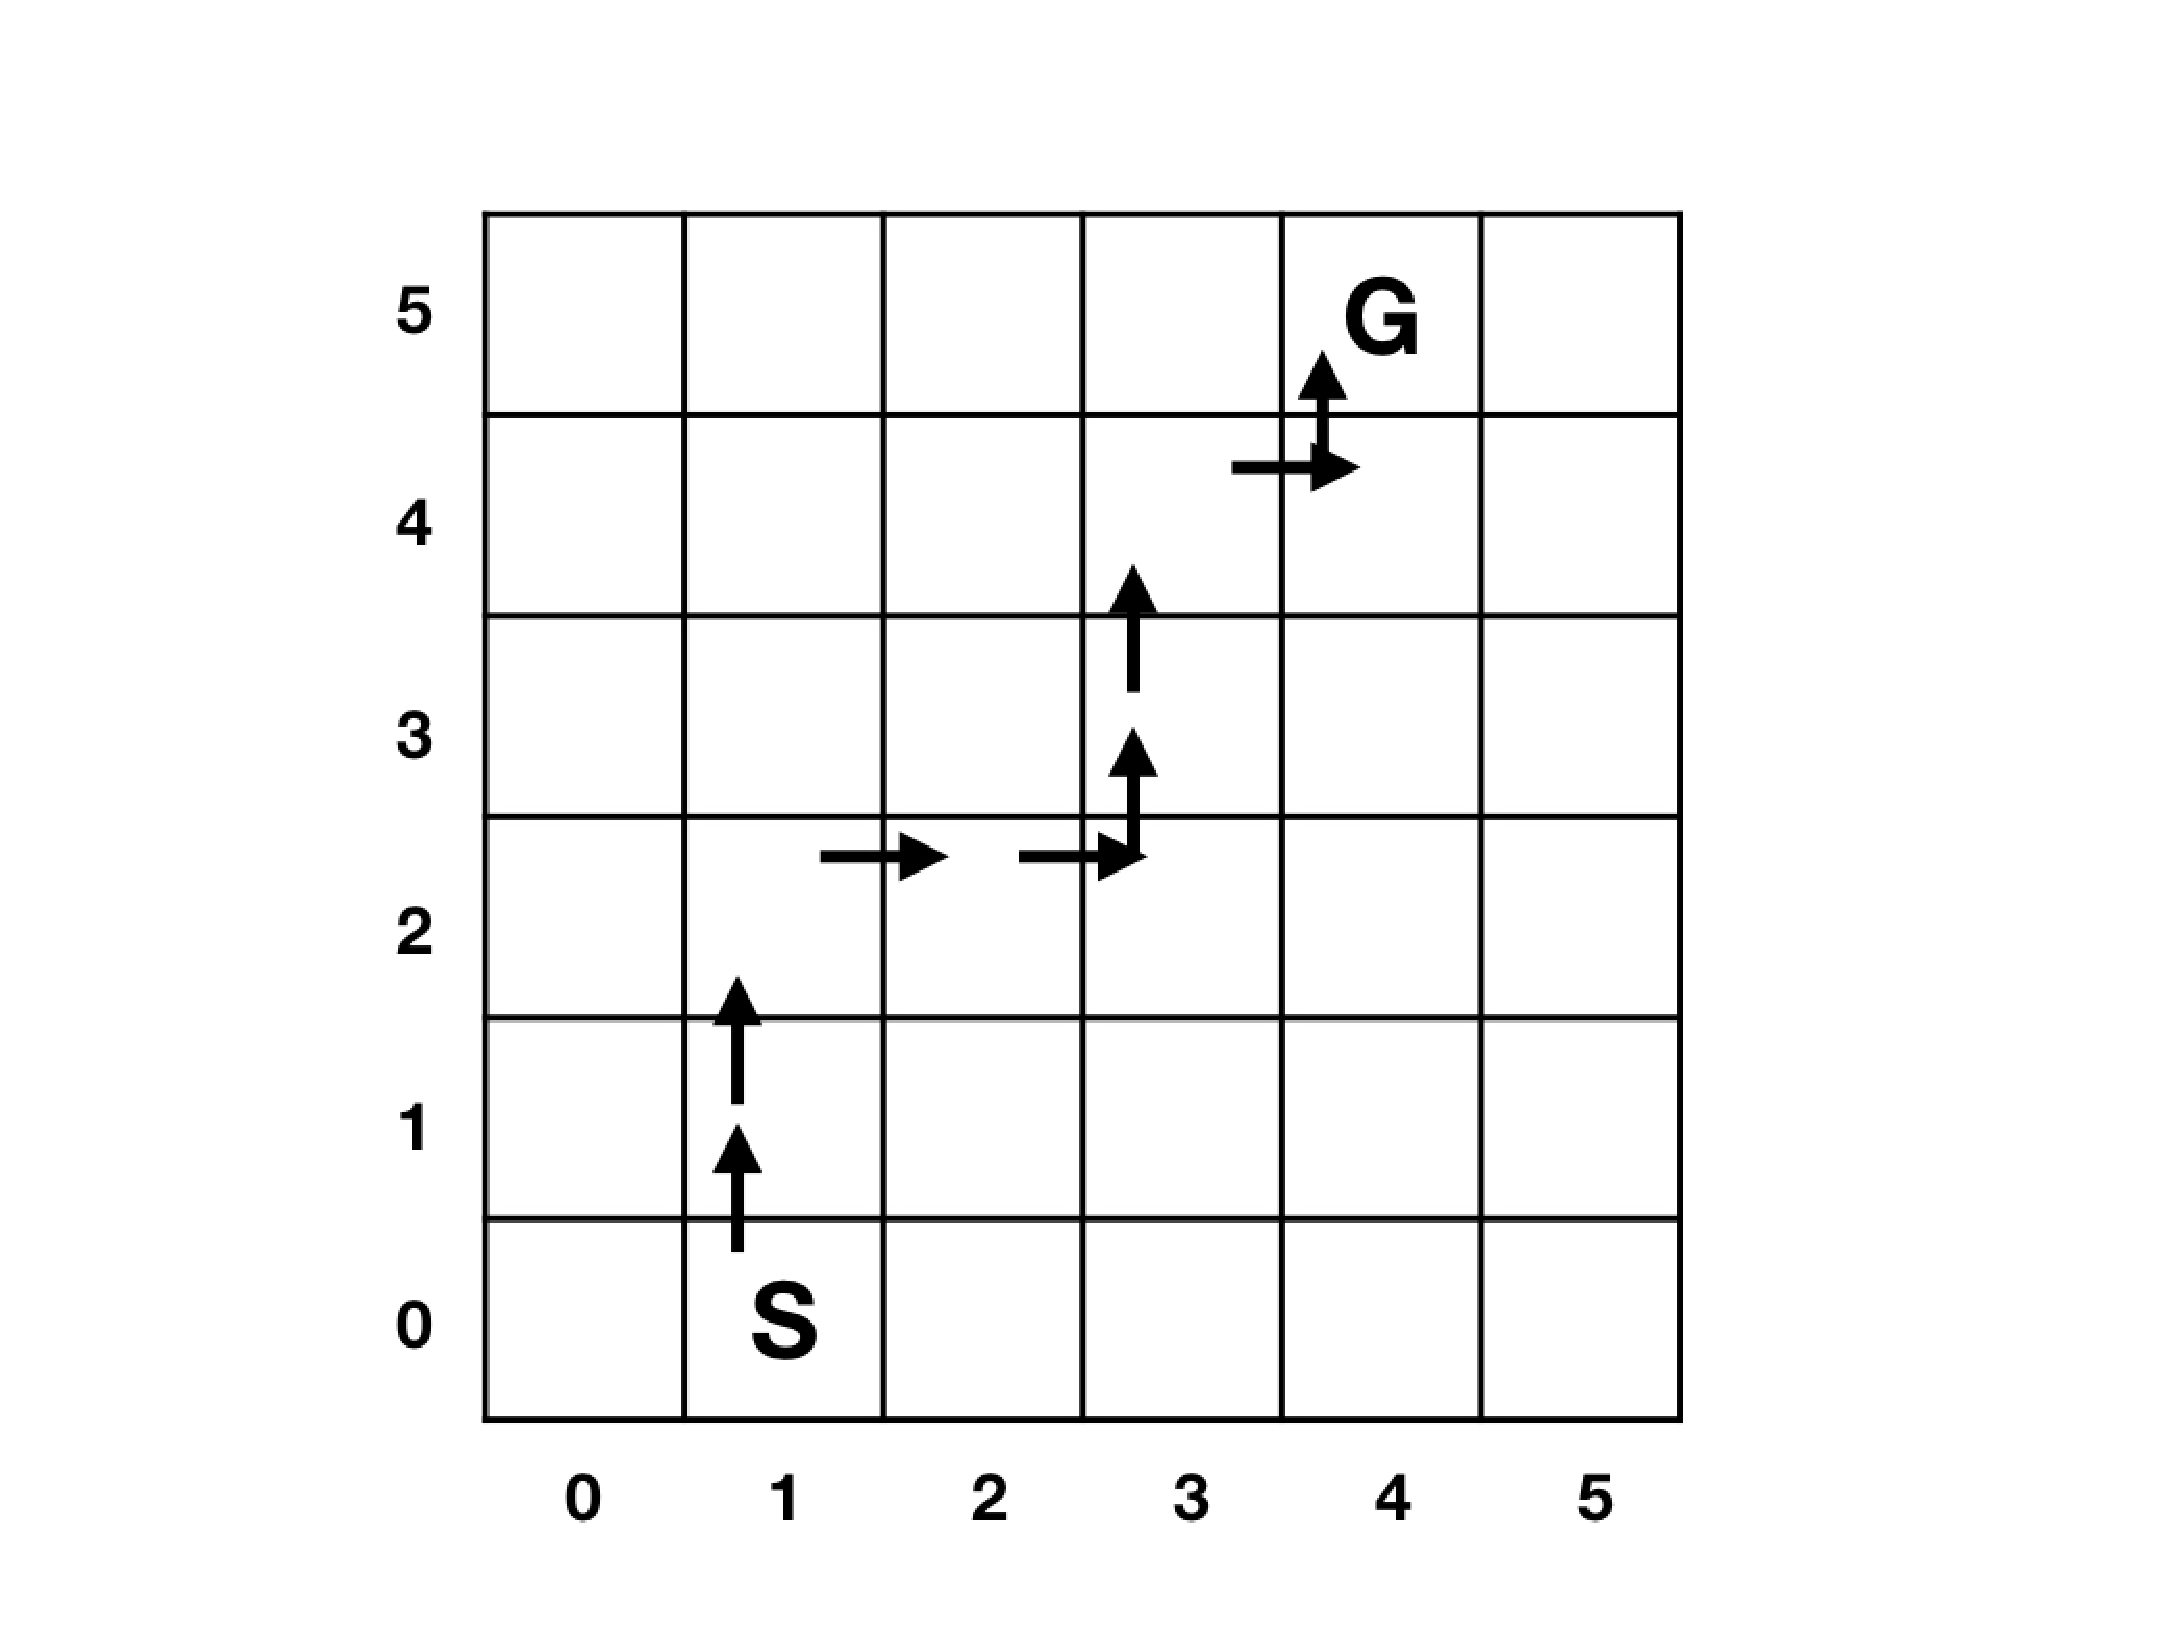
\includegraphics[clip,width = 13.0cm]{assets/rein_simple.eps}
    \caption{強化学習による最短経路検索の結果}  \label{ShortenRouteML}
\end{figure}
  


\section{地図データを活用した強化学習}

地図データを深層強化学習に応用した例がある. ~\cite{github1} しかし, これは地図をグリッドに区切りグリッド内の道をグリッド上の線に近似するという物である.
例えば, 図~\ref{gridroute}のように地点SからGまでの最短距離を選択する場合は矢印にそったグリッド上の線は選択され, これに最も近い道を選択するという物である.

しかし、この方法は高速道路などの本数の少ない道路のみであれば有効性があるが, より複雑かつ細かい都市の道路網を表現するには不十分である.

\begin{figure}[H]
    \centering
    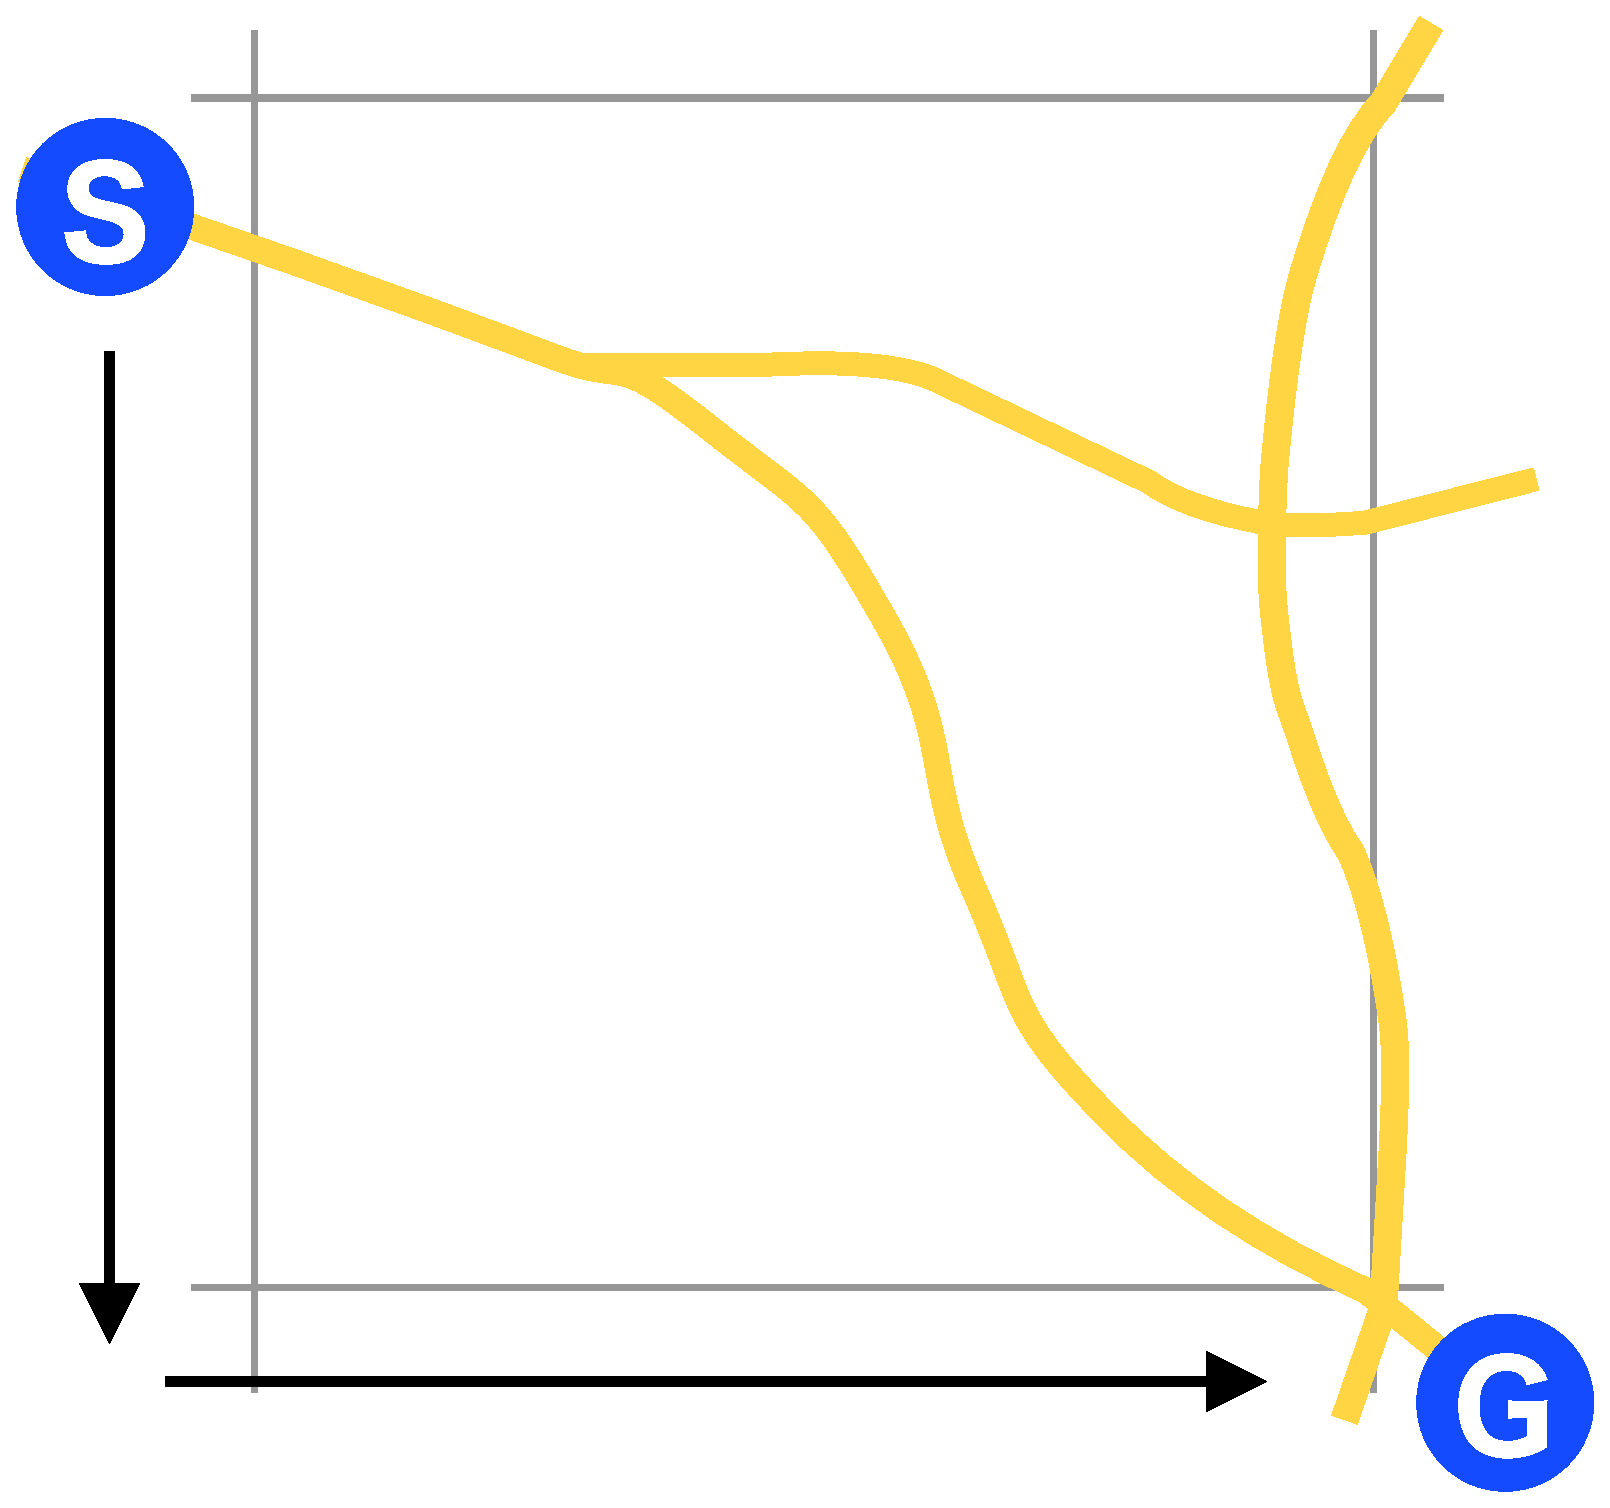
\includegraphics[clip,height = 8.0cm]{assets/GridRouteVector.eps}
    \caption{グリッドベースの地図データの近似} \label{gridroute}
\end{figure}
%% \subsection{ケース策定}   とりあえず仮綴では保留

%% 人間の目的を達成するために  とりあえず仮綴では保留


\section{仮説}

Deep Q Nueral Networkにより学習を繰り返すことで, シミュレーターないでのないでの利用者に最も最適化された経路選択を行うようになると考えた.


%%% Local Variables:
%%% mode: japanese-latex
%%% TeX-master: "./thesis"
%%% End:
